\section{Results}
\label{sec:results}

All results come from the recorded artifacts named in the generated macro file, and a value that
an artifact does not contain is printed as \NotAvailable. The study is terrain only: the radar
products were decoded, but no radar pair was qualified and no radar distance enters any ranking.

\subsection{Encoder probes on test blocks}
\label{sec:results-ml}

The encoder would be accepted as a third distance family only if, on test blocks, the lower bound of
the physics probe \Rsq{} reaches \GFivePhysRMin{} for relief $\ln \nu$ at every lag, the morphology
probe gains at least \GFiveMorphGainMin{} in \Rsq{} over a ridge on the fingerprint for the Moon or
Mars, a logistic body probe stays at or below a balanced accuracy of \GFiveBodyAccMax, the Spearman
correlation between embedding and fingerprint distances reaches \GFiveRhoMin, the top twenty
neighbours agree across seeds with a Jaccard index of at least \GFiveJaccardMin, and the encoder
beats both frozen image baselines on the two probes with paired bootstrap intervals that exclude zero, the morphology gain having a positive lower bound, and the exported model matches the training model within the parity tolerance. These acceptance criteria were fixed in the
configuration before training. Table~\ref{tab:probes} reports the probes from the evaluation
record. The encoder is reported as experimental and every ranking in this paper uses the fingerprint alone. The physics probe passes its threshold; the body probe, the agreement with the fingerprint and the seed stability are reported with their thresholds in the table; and the morphology gain and the comparison with the image baselines are not available, because they were not evaluated.

The physics probe passes its threshold: the smallest lower bound of the relief \Rsq{} over the lags is \EncoderPhysRReliefMin. But an untrained copy of the same network reaches a smallest lower bound of \RandomPhysRReliefMin, so a linear readout of the fingerprint from these windows does not show that training added anything. The body probe classifies the body with a balanced accuracy of \EncoderBodyAcc{} (interval \EncoderBodyAccLow{} to \EncoderBodyAccHigh), above the threshold of \GFiveBodyAccMax{} and close to the \NoAdvBodyAcc{} of the run without gradient reversal, so the adversarial head at the trained weight did not remove body information. Agreement between embedding distances and fingerprint distances is \EncoderAgreementRho{} (interval \EncoderAgreementLow{} to \EncoderAgreementHigh), against \RandomAgreementRho{} for the untrained network: training moved the embedding away from the physics that the fingerprint measures. The top twenty Earth neighbours agree across seeds with a mean Jaccard index of \EncoderSeedJaccard, above the \RandomSeedJaccard{} of a random ranking but below the threshold. The morphology probe and the comparison with the ImageNet and DINO baselines are not available: no crater labels were built and the baseline weights were not obtained, so neither was evaluated. At this reduced scope the paper makes no claim for learned similarity. The model report is built in the model card form of \citet{mitchell2019}, with intended use, evaluation conditions and limitations stated beside the metrics.

The browser export can be checked independently of the embedding quality. An ONNX export of the backbone of the first main run (opset \OnnxOpset; training run status in the export record: \OnnxSourceStatus) reproduces the training model on \OnnxParityN{} validation windows with a largest absolute difference of \OnnxFpDiff{} in single precision (tolerance \OnnxFpThreshold) and a smallest cosine similarity of \OnnxHalfCosine{} in half precision (tolerance \OnnxHalfThreshold), for a half precision file of \OnnxHalfBytes{} bytes. This shows that the exported graph computes the same function; it says nothing about the quality of the embedding. The web probe's own check runs the half precision file in ONNX Runtime Web \WasmOrtVersion{} under \WasmRuntime{} with \WasmThreads{} thread on \WasmWindows{} windows, with a smallest cosine similarity to the single precision Python model of \WasmMinCosine{} (tolerance \WasmThreshold) and \WasmMs{} ms per window; that timing comes from Node.js, not from a browser on a typical laptop.

\begin{table}[tbp]
\centering
\caption{Probes on test blocks. Physics: the smallest lower bound of the probe \Rsq{} over the
relief lags. Morphology: the \Rsq{} gain over the fingerprint ridge. Body: balanced accuracy of the
body probe, where chance is one third. Agreement: Spearman correlation of embedding and fingerprint
distances on cross body pairs. Seeds: mean Jaccard index of the top twenty Earth neighbours across
seeds, against \RandomSeedJaccard{} for a random ranking. Not available marks a probe that was not
evaluated.}
\label{tab:probes}
\footnotesize
\begin{tabular}{@{}lccccc@{}}
\toprule
Representation & Physics & Morphology & Body & Agreement & Seeds \\
\midrule
Random initialisation & \RandomPhysRReliefMin{} & \NotAvailable{} & \RandomBodyAcc{} & \RandomAgreementRho{} & \NotAvailable{} \\
ImageNet ResNet & \ResNetPhysRReliefMin{} & \NotAvailable{} & \NotAvailable{} & \NotAvailable{} & \NotAvailable{} \\
DINO & \DinoPhysRReliefMin{} & \NotAvailable{} & \NotAvailable{} & \NotAvailable{} & \NotAvailable{} \\
Terraluna encoder & \EncoderPhysRReliefMin{} & \EncoderMorphGain{} & \EncoderBodyAcc{} & \EncoderAgreementRho{} & \EncoderSeedJaccard{} \\
No gradient reversal & \VarLambdaZeroPhysR{} & \NotAvailable{} & \NoAdvBodyAcc{} & \VarLambdaZeroRho{} & \NotAvailable{} \\
\midrule
Acceptance threshold & \GFivePhysRMin{} & \GFiveMorphGainMin{} & \GFiveBodyAccMax{} & \GFiveRhoMin{} & \GFiveJaccardMin{} \\
\bottomrule
\end{tabular}
\end{table}

\subsection{Cross body retrieval for the lunar target}
\label{sec:results-moon}
\label{sec:results-retrieval}

The lunar target window was compared with \ComparedCount{} eligible Earth windows from the two
declared regions. Only the relief and texture distances of Equation~\eqref{eq:distance} were
comparable; no radar distance exists (Section~\ref{sec:results-radar}) and the encoder distance was
not evaluated, so both are not available. Over the compared windows the relief distance ranges from \ReliefDistanceMin{} to
\ReliefDistanceMax{} with a median of \ReliefDistanceMedian, and the texture distance from
\TextureDistanceMin{} to \TextureDistanceMax{} with a median of \TextureDistanceMedian. The first
Pareto layer holds \ShortlistCount{} window, \texttt{\ShortlistWindow} at Holuhraun, with a relief
distance of \BestReliefDistance{} and a texture distance of \BestTextureDistance. When the target
is replaced by each of its \BestCloneN{} error clones, the relief distance stays between
\BestCloneReliefMin{} and \BestCloneReliefMax, and the window ranks first by relief in
\BestRankFirstCount{} of \BestRankFirstN{} clone runs. The rank is also unchanged when the land
cover rule is tightened moderately or only the Holuhraun region is searched; when every analysis
cell must be in an allowed class, or only Rosamond Dry Lake is searched, the window leaves the
evaluated set. This stability is a frequency over the published height error model, not a
probability that the window is an analog. It mostly shows that the clones move the target's
statistics very little. The relief distance has a percentile of \BestBackgroundPercentile{} in the Earth background, which holds only the \MoonBackgroundN{} windows of the search universe rather than the \MoonBackgroundRequested{} requested. The target reference set, the distances between the target and the other \BestReferenceSpreadN{} eligible windows of its site, has a median of \MoonRefReliefMedian{} and a maximum of \MoonRefReliefMax{} in relief, so the nearest Earth window is farther from the target than every other window of the target site.

Figure~\ref{fig:candidate-distances} shows the two distances for every compared window.

\begin{figure}[tbp]
\centering
\begin{tikzpicture}
\begin{axis}[tlplot, width=0.55\linewidth, height=0.42\linewidth,
  xlabel={relief distance (RMS of $\ln \nu$)}, ylabel={texture distance (RMS of $\ln \nu$)},
  xmin=0, ymin=0, legend pos=outer north east, legend cell align=left]
% Generated by paper/scripts/tables.py. Do not edit; run make -C paper tables.
% Source: outputs/comparisons/moon-cr-site01-w000.json sha256 8a5c12462d0d5564584ce3fdaea9a3c00ca6c6f001e8ddde4c715bb793871e07.
% Source: outputs/search/targets.json sha256 6ab65f388126b3b1f4bbfe5cb59bc3b158ef623199b5222663500e1c9c0ec9d9.
% Windows without both distances, left out: 0.
\addplot[only marks, okvermilion, mark=square*, mark size=1.6pt] coordinates {(1.7103,2.1146) (2.6795,2.8724) (3.3006,3.7881) (3.3723,3.8108) (3.3122,3.5739) (2.5290,2.7505) (1.3751,1.5010) (1.9633,2.2063) (3.0404,3.2224) (3.2271,3.4904) (3.1534,3.3744) (3.2033,3.3960) (2.9339,3.1195) (2.4922,2.7706) (2.4427,2.6004) (3.0315,3.2186) (3.2184,3.4022) (3.1280,3.2881) (3.1985,3.3525) (3.0645,3.0993) (2.7731,2.8133) (1.4842,1.5139) (1.7927,1.7914) (2.9413,3.0978) (3.3524,3.7170) (3.1603,3.3684) (2.4983,2.4663) (1.2076,1.2506) (0.8811,0.9162) (1.0914,1.0901) (1.4236,1.4178) (1.4521,1.4345) (1.7980,1.7927) (1.5877,1.5599) (0.9693,1.0995) (0.6958,0.7007) (0.7552,0.7352) (0.6785,0.6585) (0.7401,0.7660) (1.1291,1.1352) (1.5156,1.4823) (1.1070,1.2541)};
\addlegendentry{Holuhraun}
\addplot[only marks, okgreen, mark=triangle*, mark size=1.6pt] coordinates {(4.1419,4.7567) (1.6266,1.6311) (2.2199,2.1933) (2.6056,2.6747) (1.2372,1.2624) (4.1904,4.4174) (1.9721,1.9818) (1.6234,1.7605) (1.6603,1.7524) (1.6765,1.6606) (2.5196,2.5766) (4.7009,4.6727) (2.0629,2.0637) (1.7136,1.9051) (1.4403,1.5554) (1.3957,1.3824) (2.4898,2.6728) (4.9495,4.9205) (2.5926,2.6719) (1.8258,2.3993) (1.3154,1.3357) (1.4252,1.4352) (2.3253,2.4840) (3.8983,3.9413) (2.3915,2.6289) (1.7330,2.4006) (1.3956,1.3762) (1.6216,1.6324) (2.0453,2.1116)};
\addlegendentry{Rosamond Dry Lake}
\addplot[only marks, mark=o, mark size=4pt, thick, black] coordinates {(0.6785,0.6585)};
\addlegendentry{first Pareto layer}

\end{axis}
\end{tikzpicture}
\caption{Derived relief and texture distances of the \ComparedCount{} compared Earth windows to the
lunar target window, by search region, from the comparison record of the target. The circled window
forms the first Pareto layer. Smaller is closer in each distance; the two are never summed. Drawn by
\texttt{paper/scripts/tables.py} from the committed comparison and target records.}
\label{fig:candidate-distances}
\end{figure}


We inspected this window as a counterexample. The target is one broad massif whose relief keeps growing with
lag, while the candidate is a mostly flat plain crossed by narrow ridges and a trough, whose
relief is close to the target's at the shortest lags but grows much more slowly with lag. Equation~\eqref{eq:distance} averages over lags and does not read the Hurst exponent, so a
window that matches at short lags can rank first against a target that is rougher at long lags.
The shortlisted window is therefore the nearest window in this terrain metric among the evaluated
windows, a candidate window identified by this search, and not a morphological analog of
Connecting Ridge.

Table~\ref{tab:first-pair} and Figure~\ref{fig:structure-functions} show the fingerprints behind
these distances for the target and for the first Earth window that was paired with it, the window
that contains the decoded radar scene centre. The lunar window is much rougher at every lag: its
relief $\nu$ grows from \MoonTargetReliefNuShort\,m to \MoonTargetReliefNuLong\,m over the lags,
against \EarthCardReliefNuShort\,m to \EarthCardReliefNuLong\,m at Holuhraun, which gives this pair
a relief distance of \FirstReliefDistance{} and a texture distance of \FirstTextureDistance. The
Hurst exponents of the lunar window, \MoonTargetReliefH{} for relief and \MoonTargetTextureH{} for
texture, lie near the highland median of \citet{rosenburg2011}, although their baselines and
estimator differ from ours. Removing the plane barely changes the lunar statistics, while it
lowers the Holuhraun texture exponent to \EarthCardTextureH, so at the longer lags much of this window's relief comes from its regional tilt. Holuhraun lava facies have been studied with UAVSAR CPR as a measure of radar roughness \citep{tolometti2022holuhraun}, yet at the hectometre scale of this fingerprint it is
far smoother than the lunar target. Radar scattering and the fingerprint describe different scales
of one surface, and this study ranks on the fingerprint only.

\begin{table}[tbp]
\centering
\caption{Derived fingerprints of the lunar target window and the first paired Earth window, on the
\ConfigGridM\,m grid over the \ConfigWindowM\,m window. $\nu$ is given at the shortest and longest
configured lag.}
\label{tab:first-pair}
\footnotesize
\begin{tabular}{@{}lcccccc@{}}
\toprule
Window & relief $\nu$ short & relief $\nu$ long & texture $\nu$ short & texture $\nu$ long & $H$ relief & $H$ texture \\
\midrule
Moon, target & \MoonTargetReliefNuShort{} & \MoonTargetReliefNuLong{} & \MoonTargetTextureNuShort{} & \MoonTargetTextureNuLong{} & \MoonTargetReliefH{} & \MoonTargetTextureH{} \\
Earth, Holuhraun & \EarthCardReliefNuShort{} & \EarthCardReliefNuLong{} & \EarthCardTextureNuShort{} & \EarthCardTextureNuLong{} & \EarthCardReliefH{} & \EarthCardTextureH{} \\
\bottomrule
\end{tabular}
\end{table}

\begin{figure}[tbp]
\centering
\begin{tikzpicture}
\begin{loglogaxis}[tlplot, width=0.62\linewidth, height=0.42\linewidth,
  xlabel={lag $L$ (m)}, ylabel={$\nu(L)$ (m)},
  xtick={270,360,540,720,1080}, xticklabels={270,360,540,720,1080},
  log ticks with fixed point, legend pos=outer north east, legend cell align=left]
\addplot[okblue, thick, mark=*] coordinates {(270,\PlotMoonReliefNuOne) (360,\PlotMoonReliefNuTwo) (540,\PlotMoonReliefNuThree) (720,\PlotMoonReliefNuFour) (1080,\PlotMoonReliefNuFive)};
\addlegendentry{Moon, relief}
\addplot[okblue, thick, dashed, mark=o] coordinates {(270,\PlotMoonTextureNuOne) (360,\PlotMoonTextureNuTwo) (540,\PlotMoonTextureNuThree) (720,\PlotMoonTextureNuFour) (1080,\PlotMoonTextureNuFive)};
\addlegendentry{Moon, texture}
\addplot[okvermilion, thick, mark=square*] coordinates {(270,\PlotEarthReliefNuOne) (360,\PlotEarthReliefNuTwo) (540,\PlotEarthReliefNuThree) (720,\PlotEarthReliefNuFour) (1080,\PlotEarthReliefNuFive)};
\addlegendentry{Earth, relief}
\addplot[okvermilion, thick, dashed, mark=square] coordinates {(270,\PlotEarthTextureNuOne) (360,\PlotEarthTextureNuTwo) (540,\PlotEarthTextureNuThree) (720,\PlotEarthTextureNuFour) (1080,\PlotEarthTextureNuFive)};
\addlegendentry{Earth, texture}
\end{loglogaxis}
\end{tikzpicture}
\caption{Structure functions of the primary lunar target window (Site01 of PGDA product 78,
window \texttt{moon-sps-x2-y2}) and the first paired Earth window (Copernicus GLO-30,
\texttt{earth-utm27n-e280-n2880}, Holuhraun), on the \ConfigGridM\,m analysis grid, from the
windows evidence record of the gate G0 pilot. Solid lines are relief (raw heights) and dashed lines
texture (best fit plane removed). Each curve is the equal weight mean over the two grid axes. The
slopes give the Hurst exponents of Table~\ref{tab:first-pair}. The Earth window was chosen because
it contains the decoded radar scene centre, not by similarity.}
\label{fig:structure-functions}
\end{figure}


Figure~\ref{fig:hillshades} shows the two windows of the shortlist pair. The lunar window spans
\HillMoonRelief\,m of relief in a cratered massif, and the Earth window spans \HillEarthRelief\,m
at the edge of the Holuhraun region, with a flat floor between narrow ridges. The pair is the closest
in the evaluated set by both distances, yet the hillshades differ in morphology, which is the kind
of difference that a second order fingerprint does not capture and that the encoder is meant to test.

\begin{figure}[tbp]
\centering
\begin{tikzpicture}
  \node[inner sep=0, anchor=south west] (moon) at (0,0)
    {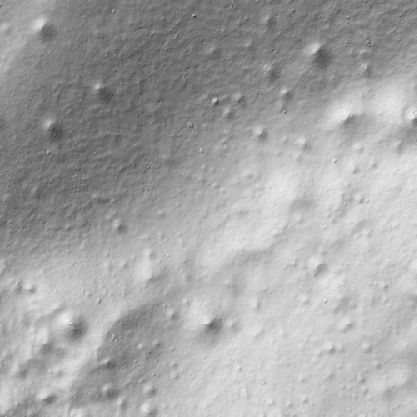
\includegraphics[width=0.42\linewidth]{figures/generated/hillshade-moon.pdf}};
  \node[inner sep=0, anchor=south west] (earth) at ([xshift=0.06\linewidth]moon.south east)
    {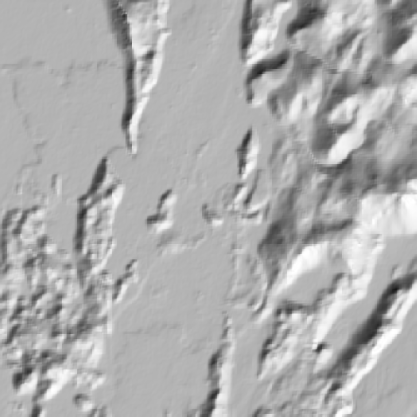
\includegraphics[width=0.42\linewidth]{figures/generated/hillshade-earth.pdf}};
  \foreach \panel in {moon, earth} {
    \draw[line width=0.4pt] (\panel.south west) rectangle (\panel.north east);
    \fill[white, opacity=0.8] ([xshift=4pt, yshift=4pt]\panel.south west)
      rectangle ([xshift={4pt+0.084\linewidth+6pt}, yshift=17pt]\panel.south west);
    \draw[line width=1.2pt] ([xshift=7pt, yshift=8pt]\panel.south west)
      -- ([xshift={7pt+0.084\linewidth}, yshift=8pt]\panel.south west);
    \node[font=\footnotesize, anchor=south] at ([xshift={7pt+0.042\linewidth}, yshift=8pt]\panel.south west) {1 km};
    \draw[-{Stealth[length=4pt]}, line width=0.6pt] ([xshift=-9pt, yshift=-22pt]\panel.north east)
      -- ([xshift=-9pt, yshift=-6pt]\panel.north east);
  }
  \node[font=\footnotesize, anchor=north] at ([xshift=-9pt, yshift=-22pt]moon.north east) {$+y$};
  \node[font=\footnotesize, anchor=north] at ([xshift=-9pt, yshift=-22pt]earth.north east) {N};
  \node[font=\footnotesize, anchor=north] at ([yshift=-2pt]moon.south) {(a) Moon, Connecting Ridge target window};
  \node[font=\footnotesize, anchor=north] at ([yshift=-2pt]earth.south) {(b) Earth, shortlisted Holuhraun window};
\end{tikzpicture}
\caption{Hillshades of the lunar target window and the shortlisted Earth window, each
\ConfigWindowM\,m wide, lit from azimuth \HillAzimuth{} degrees at \HillAltitude{} degrees altitude with no vertical
exaggeration. (a) Window \texttt{moon-sps-x2-y2}, centred at latitude \HillMoonLat{} and longitude \HillMoonLon{}
degrees, from the 5 m surface heights of PGDA product 78 Site01 \citep{barker2021}, shown at every
second pixel in the product's south polar stereographic grid; the arrow is grid north ($+y$). Most
5 m pixels are interpolated between LOLA tracks (Section~\ref{sec:data}). (b) Window
\texttt{earth-utm27n-e285-n2879}, centred at latitude \HillEarthLat{} and longitude \HillEarthLon{} degrees, resampled
from Copernicus GLO-30 tile N64 W017 \citep{airbus2022copernicus} onto a 10 m grid about its centre
with the window resampler; the arrow is north. Generated by \texttt{paper/scripts/figures.py},
which records the input digests.}
\label{fig:hillshades}
\end{figure}


The same gap holds across bodies. Over the windows that the search read, the relief $\ln \nu$ distributions of the lunar site and of Earth overlap with a coefficient of \OverlapEarthMoonNuShort{} at the shortest lag and \OverlapEarthMoonNuLong{} at the longest, while the Martian and Earth samples overlap at \OverlapEarthMarsNuShort{} and \OverlapEarthMarsNuLong{} (Appendix~\ref{sec:appendix-data-analysis}). At the longest lag no evaluated Earth window falls in the range of the lunar site, so for this target the shortlist names the least different window rather than a similar one.

\subsection{Cross body retrieval for the Martian targets}
\label{sec:results-mars}

Two Martian target windows were fixed by rules declared before ranking. At Jezero crater, the primary window is the eligible window nearest the landing site of the Perseverance rover on the CTX model in the declared box that passes the quality threshold; its site has \JezeroTargetEligible{} eligible of \JezeroTargetGenerated{} generated windows. In Arcadia Planitia, it is the eligible window nearest the centre of the CTX model that passes the threshold nearest the box centre, with \ArcadiaTargetEligible{} eligible of \ArcadiaTargetGenerated{} windows. Each was compared with the same \JezeroCompared{} Earth windows as the lunar target (Figure~\ref{fig:candidate-distances}).

The Martian targets sit much closer to the Earth sample than the lunar target. For Jezero the first Pareto layer holds \JezeroShortlistSize{} windows, with relief distances from \JezeroShortReliefMin{} to \JezeroShortReliefMax{} and texture distances from \JezeroShortTextureMin{} to \JezeroShortTextureMax, against a median relief distance of \JezeroReliefMedian{} over all compared windows. For Arcadia it holds \ArcadiaShortlistSize{} windows, with relief distances from \ArcadiaShortReliefMin{} to \ArcadiaShortReliefMax{} and texture distances from \ArcadiaShortTextureMin{} to \ArcadiaShortTextureMax, against a median of \ArcadiaReliefMedian. These shortlisted distances lie below the median internal distance of each Martian site, whose target reference sets have median relief distances of \JezeroRefReliefMedian{} at Jezero and \ArcadiaRefReliefMedian{} at Arcadia, so under this fingerprint the shortlisted Earth windows lie within the spread of windows of the target sites themselves. The lowest background percentile of a compared window is \JezeroBgPctMin{} for Jezero and \ArcadiaBgPctMin{} for Arcadia, again over a background of only the \JezeroBackgroundN{} windows of the search universe. The Martian models have no published error clones, so these distances carry no measurement error spread, and no counterexample inspection was recorded for the Martian shortlists. The shortlisted windows are candidate windows identified by this search for the two Martian targets, with the same caveat as for the Moon: a small distance at hectometre lags says nothing about morphology, block sizes or the surface at the scale of a rover.

\subsection{Model variations}
\label{sec:results-variations}

Table~\ref{tab:variations} lists the planned variations of the encoder, in the manner of a model
variations table, with the results that the evaluation record holds for each.

\begin{table}[tbp]
\centering
\caption{Encoder variations, from the evaluation record where it exists. Physics, body and agreement as in
Table~\ref{tab:probes}.}
\label{tab:variations}
\footnotesize
\begin{tabular}{@{}lccc@{}}
\toprule
Variation & Physics & Body & Agreement \\
\midrule
Main configuration & \VarMainPhysR{} & \VarMainBodyAcc{} & \VarMainRho{} \\
No physics head & \VarNoPhysPhysR{} & \VarNoPhysBodyAcc{} & \VarNoPhysRho{} \\
No gradient reversal & \VarLambdaZeroPhysR{} & \VarLambdaZeroBodyAcc{} & \VarLambdaZeroRho{} \\
Weaker gradient reversal & \VarLambdaTenthPhysR{} & \VarLambdaTenthBodyAcc{} & \VarLambdaTenthRho{} \\
Stronger gradient reversal & \VarLambdaOnePhysR{} & \VarLambdaOneBodyAcc{} & \VarLambdaOneRho{} \\
VICReg only & \VarVicregOnlyPhysR{} & \VarVicregOnlyBodyAcc{} & \VarVicregOnlyRho{} \\
Physics head only & \VarPhysOnlyPhysR{} & \VarPhysOnlyBodyAcc{} & \VarPhysOnlyRho{} \\
\bottomrule
\end{tabular}
\end{table}

\subsection{Benchmarks}
\label{sec:benchmarks}

\paragraph{Validation sweep.} After the test evaluation above, we trained additional runs and
evaluated them, together with the earlier runs, on the validation blocks only; the test blocks were
not read again, and no number in this subsection was used to select a model on test. The probes are
those of Table~\ref{tab:probes}, with one caveat recorded in the evaluation record: the ridge
penalty of the probes was chosen on the same validation rows that are scored, so these values are
optimistic. Table~\ref{tab:benchmarks} lists every run. Three findings hold across the table. The
body probe stays between \ValFortyCBody{} and \ValLamZeroSBody{} for every trained run, whatever the
adversarial weight, including the run without gradient reversal, so the adversary at these weights
does not remove body information; every value lies above the acceptance threshold of
\GFiveBodyAccMax. The untrained network reaches a physics probe of \ValRandomSPhys{} and an agreement
of \ValRandomSRho, against at most \ValLamThreeSBRho{} for any trained run: training lowers the
agreement between embedding and fingerprint distances instead of raising it. And training the
main configuration for \ThruMpsFortyEpochs{} rather than \TrainEpochs{} epochs lowers the agreement
of every seed, from \ValLamThreeSCRho{} to \ValLamThreeSBRho{} at \TrainEpochs{} epochs to
\ValFortyCRho{} to \ValFortyARho{} at \ThruMpsFortyEpochs{} epochs. The mean Jaccard index of the
top twenty Earth neighbours across three seeds is \ValFortyJaccard{} for the
\ThruMpsFortyEpochs{} epoch runs and \ValSweepJaccard{} for the \TrainEpochs{} epoch group
\texttt{\ValSweepJaccardArm}, against \ValSweepRandomJaccard{} for a random ranking; both rest on a
single target window, and the two groups differ in adversarial weight as well as in length, so they
do not isolate the effect of training length.

\begin{table}[tbp]
\centering
\caption{Validation benchmark of the encoder (\ValSweepParams{} backbone parameters). Validation
blocks only; the probe penalty was chosen on the scored rows, so the values are optimistic. Physics:
smallest lower bound of the relief probe \Rsq{} over the lags. Body: balanced accuracy of the body
probe, where chance is one third. Agreement: Spearman correlation of embedding and fingerprint
distances. $\lambda_{\max}$ is the adversarial weight of Equation~\eqref{eq:total}.}
\label{tab:benchmarks}
\footnotesize
\begin{tabular}{@{}lcccccc@{}}
\toprule
Run & $\lambda_{\max}$ & Epochs & Seed & Physics & Body & Agreement \\
\midrule
Untrained network & & 0 & 0 & \ValRandomSPhys{} & \ValRandomSBody{} & \ValRandomSRho{} \\
No gradient reversal & 0 & \TrainEpochs{} & 0 & \ValLamZeroSPhys{} & \ValLamZeroSBody{} & \ValLamZeroSRho{} \\
Weaker gradient reversal & 0.1 & \TrainEpochs{} & 0 & \ValLamTenthSPhys{} & \ValLamTenthSBody{} & \ValLamTenthSRho{} \\
Main configuration & 0.3 & \TrainEpochs{} & 0 & \ValLamThreeSAPhys{} & \ValLamThreeSABody{} & \ValLamThreeSARho{} \\
Main configuration & 0.3 & \TrainEpochs{} & 1 & \ValLamThreeSBPhys{} & \ValLamThreeSBBody{} & \ValLamThreeSBRho{} \\
Main configuration & 0.3 & \TrainEpochs{} & 2 & \ValLamThreeSCPhys{} & \ValLamThreeSCBody{} & \ValLamThreeSCRho{} \\
Stronger gradient reversal & 1 & \TrainEpochs{} & 0 & \ValLamOneSAPhys{} & \ValLamOneSABody{} & \ValLamOneSARho{} \\
Stronger gradient reversal & 1 & \TrainEpochs{} & 1 & \ValLamOneSBPhys{} & \ValLamOneSBBody{} & \ValLamOneSBRho{} \\
Stronger gradient reversal & 1 & \TrainEpochs{} & 2 & \ValLamOneSCPhys{} & \ValLamOneSCBody{} & \ValLamOneSCRho{} \\
No physics head & 0.3 & \TrainEpochs{} & 0 & \ValNoPhysSPhys{} & \ValNoPhysSBody{} & \ValNoPhysSRho{} \\
Main configuration, longer & 0.3 & \ThruMpsFortyEpochs{} & 0 & \ValFortyAPhys{} & \ValFortyABody{} & \ValFortyARho{} \\
Main configuration, longer & 0.3 & \ThruMpsFortyEpochs{} & 1 & \ValFortyBPhys{} & \ValFortyBBody{} & \ValFortyBRho{} \\
Main configuration, longer & 0.3 & \ThruMpsFortyEpochs{} & 2 & \ValFortyCPhys{} & \ValFortyCBody{} & \ValFortyCRho{} \\
\midrule
Acceptance threshold & & & & \GFivePhysRMin{} & \GFiveBodyAccMax{} & \GFiveRhoMin{} \\
\bottomrule
\end{tabular}
\end{table}

\paragraph{Training throughput.} The run records give the measured training throughput per epoch at
a batch of \TrainBatch{} with the same model and data. On a server with \ThruCpuCount{} virtual
CPUs, the first main run trained at a median of \ThruCpuMedian{} windows per second (\ThruCpuMin{}
to \ThruCpuMax{} over its epochs). On a laptop accelerator through the PyTorch Metal Performance
Shaders backend, a \TrainEpochs{} epoch run of the sweep trained at a median of \ThruMpsTwelveMedian{} windows per
second (\ThruMpsTwelveMin{} to \ThruMpsTwelveMax), and a \ThruMpsFortyEpochs{} epoch run at
\ThruMpsFortyMedian{} (\ThruMpsFortyMin{} to \ThruMpsFortyMax), finishing in
\ThruMpsFortyWallSeconds\,s of wall clock time. The CPU throughput varied widely between epochs,
and the records do not state why. The reduced schedule of Section~\ref{sec:training} was set for the
CPU server; on the accelerator the longer runs of Table~\ref{tab:benchmarks} took minutes, and
on validation blocks they still miss the body and agreement thresholds.

\paragraph{Browser parity.} The half precision ONNX encoder run in ONNX Runtime Web
\WasmOrtVersion{} reproduces the single precision Python model on \WasmWindows{} windows with a
smallest cosine similarity of \WasmMinCosine{} against a tolerance of \WasmThreshold, at
\WasmMs{} ms per window in \WasmRuntime{} with \WasmThreads{} thread
(Section~\ref{sec:results-ml}). The fingerprint and the window resampling have a TypeScript port
that the browser worker runs; shared fixtures hold it to the Python implementation within the
tolerances recorded in each fixture file, which are not reported here as generated values. The
latency of the fingerprint and of the encoder in a browser on typical hardware is not available,
because neither was timed in a browser.

\subsection{Held out body}
\label{sec:results-heldout}

A run trained on the Moon and Earth only and probed on Mars would test whether the physics probe transfers to a body the encoder has not seen. The evaluation record holds no such run, so the smallest relief probe \Rsq{} on held out Mars is \HeldOutMarsR.

\subsection{Radar context for the lunar target}
\label{sec:results-radar}

Both radar products were decoded, but the radar comparison was not completed, and no radar number
enters any distance. On the lunar side, the Mini-RF south polar CPR mosaic was read over the
site extent, with \MiniRFValidPixels{} valid and \MiniRFNodataPixels{} nodata pixels. The mosaic
combines east and west looking passes from several acquisitions, so the incidence angle of a pixel
is not recoverable from it, and its label does not state the transmit handedness. On the Earth
side, a region of interest of \UavsarRoiSide\,m at Holuhraun was decoded from the UAVSAR L band
covariance product, with \UavsarPixels{} valid pixels at \UavsarLooks{} nominal looks and a median
local incidence of \UavsarIncidenceMedian{} degrees. The median ratio of the handedness dependent
term to the base same sense power is \UavsarHandednessRatioMedian, but the handedness convention is
not verified against the Mini-RF convention. The radar conversions pass their checks against
independent fixtures, but the eligibility check of band, convention, geometry and support was not
run for any pair, so no radar pair is qualified, no radar distance exists, and no Earth value is
presented as equivalent to Mini-RF.

As a literature check of the Earth radar processing, we repeated the facies comparison of
\citet{tolometti2022holuhraun} on the same UAVSAR scene, with \HoluhraunValidPixels{} valid pixels
inside the mapped facies after the incidence and nodata rules of a protocol fixed before any
result was read. The median CPR is \HoluhraunRubblyMedian{} for rubbly, \HoluhraunSpinyMedian{}
for spiny and \HoluhraunUndiffMedian{} for undifferentiated lava. The pairwise distribution
overlaps are \HoluhraunOverlapRS\%, \HoluhraunOverlapRU\% and \HoluhraunOverlapSU\% (rubbly and
spiny, rubbly and undifferentiated, spiny and undifferentiated). Applied to the published radar
values of that study, the same overlap definition gives \PublishedOverlapRS\%,
\PublishedOverlapRU\% and \PublishedOverlapSU\%. Two of our three overlaps exceed the published comparators and one is slightly lower, so our facies are not markedly better separated than the published ones, which is the plausibility condition of the check, but the overlaps differ in detail; the authors' mosaic combined two data takes, their histogram binning and whether their low pass filter acts on CPR or on the covariance are not stated, and the handedness convention is not verified against theirs. The literature check is only partial, because its shadow behaviour part is unavailable without a permanent shadow product; its Holuhraun part is recorded as consistent. Mini-RF and UAVSAR also differ in band, look geometry
and processing, so even a completed comparison would show the signatures side by side rather than
as a distance.
